\chapter{Eclipse Platform}
\label{sec:EclipsePlatform}

In diesem Kapitel wird gezeigt, was Eclipse für Möglichkeiten anbietet, um eine moderne Entwicklungsumgebung zu implementieren. Diese verschiedenen Möglichkeiten werden Verglichen und die Vor- und Nachteile aufgezeigt. Es werden auch die wichtigsten Eclipse Features, welche für das Entwickeln von Eclipse Rich Client Platform (RCP) Applikationen benötigt werden, beschrieben.

\section{Eclipse als Platform}

Eclipse RCP bietet eine Basis um beliebige (nicht zwingendermassen Entwicklungsumgebungen) Betriebssystem unabhängige Applikationen zu entwickeln. Es bietet Mechanismen, wie Plugins und Extension Points, um modulares programmieren zu unterstützen und vereinfachen. Auch bietet das Framework Features, wie das Konzept von Views und Editoren und vielem mehr, welche häufig in Applikationen gebraucht werden.

\section{Plugins}

Eclipse Applikationen nützen eine auf der OSGi Speizifikation basierten Runtime, eine Komponente in dieser Runtime ist ein Plugin. Eine Eclipse RCP Applikation besteht also aus einer Ansammlung von Plugins. Ein Eclipse Plugin ist ein Modul, welches gegen aussen ein API und Extension Points anbieten kann. 

\section{Extension Points}

Um Plugins erweitern zu können, bietet Eclipse das Konzept von Extension Points an. Über Extension Points können Plugins ein bestimmte Funktionalität anbieten, welches von anderen Plugins aufgerufen werden kann. 
\newline
So existiert zum Beispiel ein Plugin, welches einen Extension Point für Views definiert. Ein anderes Plugin kann über diesen Extension Point, deklarativ in einem XML File eine neue View erstellen. \cite{extensionpoints}

\begin{figure}[H]
	\centering
		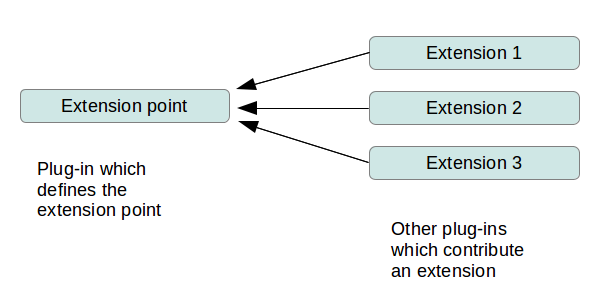
\includegraphics[scale=0.5]{platform/extensionpoint.png}
		\caption{Ein Plugin, welches einen Extension Point anbietet. Andere Plugins können}
		\captionsetup{margin=0cm,font={footnotesize}}
		\label{fig:extensionpoint}
\end{figure}

Es ist auch möglich eigene Extension Points zu definieren, falls ein eigens Plugin für andere Entwickler offen stehen soll für Erweiterungen.

\section{Eclipse basierte MCore Entwicklungsumgebung}

Eclipse als Grundlage für eine Entwicklungsumgebung zu verwenden eignet sich besonders gut, da Eclipse schon einiges an Funktionalität für eine IDE zur Verfügung stellt und schon einige Entwicklungsumgebungen mit Eclipse RCP entwickelt wurden. Auch existieren einige Tools, auf welche ich noch genauer eingehen werde, wie Xtext und DLTK, welche das entwickeln einer Entwicklungsumgebung weiter vereinfachen.

\subsection{JDT}
Eine Möglichkeit die MCore Entwicklungsumgebung zu implementieren, wäre über normalen Features (Plugins und Extension Points) von dem Eclipse Java Development Tools (JDT). Dies bringt aber einige Nachteile mit sich. Es müssten sehr viel von Hand 

\subsection{Xtext}
XText ist ein Framework, welches es erleichtert eine auf Eclipse basierte Entwicklungsumgebungen zu programmieren. Es ermöglicht auf schnelle Weise ein Grundgerüst einer IDE mit Features wie:

\begin{itemize} 
	\item Ein Editor mit Syntax Highligting
	\item Code Completion
	\item Compiler Integration
	\item Ein Java-basierter Debugger
\end{itemize}

zu generieren. \cite{xtext} Es muss lediglich eine Grammatik für die Sprache definiert werden. Der grosse Nachteil ist, dass C, inklusive Preprozessor, zu parsen sehr schwierig ist und auch mit Xtext nicht einfach zu implementieren ist.

\subsection{DLTK}
Das Dynamic Language Toolkit ist ein weiteres Framework, welches Grundgerüste für Entwicklungsumgebungen generiert. Ursprünglicherweise war das Framework nur für dynamische Sprachen geignet, es können aber auch für statische Sprachen verwendet werden. Die D

\subsection{Eclipse CDT}
Das Eclipse C-Development Tools (CDT) ist eine Eclipse Distribution mit Sprach Unterstützung für C und C++. Das CDT bietet alle Features welche man von einer Entwicklungsumgebung erwartet und stellt Extension Points zur Verfügung um diese für eine eigene Entwicklungsumgebung zu gebrauchen. So kann man mit relativ wenig Aufwand einen neues Compiler Backend in die Entwicklungsumgebung einbinden, welche den C Code kompiliert.

\subsection{Verwendung für MCore Eclipse}
Ich habe mich dazu entschieden, das Eclipse CDT als Target Platform zu wählen. Ich kann somit alle Features welche das Eclipse CDT zur Verfügung stellt brauchen und einfach mögliche Anpassungen machen. Die Frameworks, welche ein Grundgerüst einer Entwicklungsumgebung generieren funktionieren leider für C nicht vollständig und sind somit keine guten Alternativen.
